\chapter{Introduction}
\epigraphhead[120]{\epigraph{An investment in knowledge pays the best interest.}{\textit{Benjamin Franklin}}}


\textquote[{\url{http://www.bbc.co.uk/news/uk-16115139} \cite{bbc}}]{Storm caused wind turbine fire} this headline news is one which the manufacturers and designers of wind turbines try to avoid. The failure or wrong design of a wind turbine shut down mechanism can have a catastrophic consequence as shown in \Fref{fig:BBC}.

\begin{figure}[!htb]
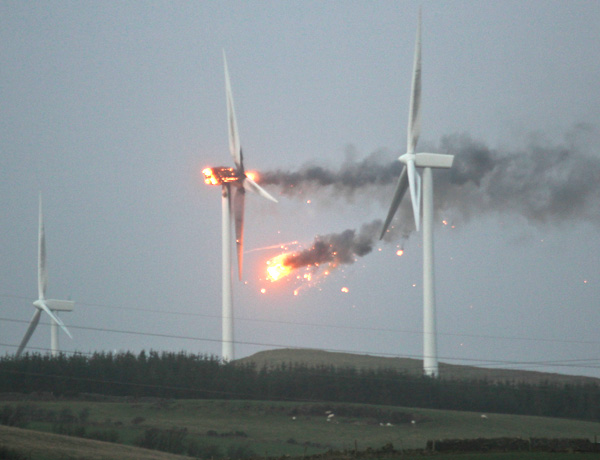
\includegraphics[width=0.84\textwidth]{BBCTurbineCrash}
\caption{Exploded wind turbine in Ardrossan, North Ayrshire, Scotland due to high winds and problems with the emergency shutdown \cite{bbc}}
\label{fig:BBC}
\end{figure}

Vector x $x$: $\mathbfit{x}$ $\mathbfit{\alpha}$   \\
Matrix X $X$: $\mathbfit{X}$ $\mathbfit{\Gamma}$    \\
Tensor x: $\mathsfbfit{x}$ $\mathsfbfit{\alpha}$ \\
Tensor X: $\mathsfbfit{X}$ $\mathsfbfit{\Gamma}$  \\

% \mathbfit  -->  sans-serif italic      --> vector and matrix symbols
% \mathsfbfit --> sans-serif bold italic --> tensor symbols


$\vec{\alpha}$ \\

% some include from inkscape pdf/LaTeX export
\begin{figure}[!htb]
	\def\svgwidth{0.84\textwidth}
	\input{intro/fig/spring-damper-example-dynamic.pdf_tex}
	\caption{Monolithic/co-simulation test problem}
	\label{fig:spring-damper-example-dynamic}
\end{figure}


Lorem ipsum dolor sit amet, consetetur sadipscing elitr, sed diam nonumy eirmod tempor invidunt ut labore et dolore magna aliquyam erat, sed diam voluptua. At vero eos et accusam et justo duo dolores et ea rebum. Stet clita kasd gubergren, no sea takimata sanctus est Lorem ipsum dolor sit amet. Lorem ipsum dolor sit amet, consetetur sadipscing elitr, sed diam nonumy eirmod tempor invidunt ut labore et dolore magna aliquyam erat, sed diam voluptua. At vero eos et accusam et justo duo dolores et ea rebum. Stet clita kasd gubergren, no sea takimata sanctus est Lorem ipsum dolor sit amet. see Definition \ref{def:field}


\begin{myDefinition}{(Physical) Field}{field}
\blockquote[{\cite{gribbin1998q}}]{
A field is a physical quantity that has a value for each point in space and time.
}
\end{myDefinition}



\begin{figure}[!htb]
	\resizebox{0.84\textwidth}{!}{% GNUPLOT: LaTeX picture with Postscript
\begingroup
  \makeatletter
  \providecommand\color[2][]{%
    \GenericError{(gnuplot) \space\space\space\@spaces}{%
      Package color not loaded in conjunction with
      terminal option `colourtext'%
    }{See the gnuplot documentation for explanation.%
    }{Either use 'blacktext' in gnuplot or load the package
      color.sty in LaTeX.}%
    \renewcommand\color[2][]{}%
  }%
  \providecommand\includegraphics[2][]{%
    \GenericError{(gnuplot) \space\space\space\@spaces}{%
      Package graphicx or graphics not loaded%
    }{See the gnuplot documentation for explanation.%
    }{The gnuplot epslatex terminal needs graphicx.sty or graphics.sty.}%
    \renewcommand\includegraphics[2][]{}%
  }%
  \providecommand\rotatebox[2]{#2}%
  \@ifundefined{ifGPcolor}{%
    \newif\ifGPcolor
    \GPcolortrue
  }{}%
  \@ifundefined{ifGPblacktext}{%
    \newif\ifGPblacktext
    \GPblacktextfalse
  }{}%
  % define a \g@addto@macro without @ in the name:
  \let\gplgaddtomacro\g@addto@macro
  % define empty templates for all commands taking text:
  \gdef\gplbacktext{}%
  \gdef\gplfronttext{}%
  \makeatother
  \ifGPblacktext
    % no textcolor at all
    \def\colorrgb#1{}%
    \def\colorgray#1{}%
  \else
    % gray or color?
    \ifGPcolor
      \def\colorrgb#1{\color[rgb]{#1}}%
      \def\colorgray#1{\color[gray]{#1}}%
      \expandafter\def\csname LTw\endcsname{\color{white}}%
      \expandafter\def\csname LTb\endcsname{\color{black}}%
      \expandafter\def\csname LTa\endcsname{\color{black}}%
      \expandafter\def\csname LT0\endcsname{\color[rgb]{1,0,0}}%
      \expandafter\def\csname LT1\endcsname{\color[rgb]{0,1,0}}%
      \expandafter\def\csname LT2\endcsname{\color[rgb]{0,0,1}}%
      \expandafter\def\csname LT3\endcsname{\color[rgb]{1,0,1}}%
      \expandafter\def\csname LT4\endcsname{\color[rgb]{0,1,1}}%
      \expandafter\def\csname LT5\endcsname{\color[rgb]{1,1,0}}%
      \expandafter\def\csname LT6\endcsname{\color[rgb]{0,0,0}}%
      \expandafter\def\csname LT7\endcsname{\color[rgb]{1,0.3,0}}%
      \expandafter\def\csname LT8\endcsname{\color[rgb]{0.5,0.5,0.5}}%
    \else
      % gray
      \def\colorrgb#1{\color{black}}%
      \def\colorgray#1{\color[gray]{#1}}%
      \expandafter\def\csname LTw\endcsname{\color{white}}%
      \expandafter\def\csname LTb\endcsname{\color{black}}%
      \expandafter\def\csname LTa\endcsname{\color{black}}%
      \expandafter\def\csname LT0\endcsname{\color{black}}%
      \expandafter\def\csname LT1\endcsname{\color{black}}%
      \expandafter\def\csname LT2\endcsname{\color{black}}%
      \expandafter\def\csname LT3\endcsname{\color{black}}%
      \expandafter\def\csname LT4\endcsname{\color{black}}%
      \expandafter\def\csname LT5\endcsname{\color{black}}%
      \expandafter\def\csname LT6\endcsname{\color{black}}%
      \expandafter\def\csname LT7\endcsname{\color{black}}%
      \expandafter\def\csname LT8\endcsname{\color{black}}%
    \fi
  \fi
  \setlength{\unitlength}{0.0500bp}%
  \begin{picture}(7200.00,5040.00)%
    \gplgaddtomacro\gplbacktext{%
      \colorrgb{0.00,0.00,0.00}%
      \put(947,755){\makebox(0,0)[r]{\strut{}-0.2}}%
      \colorrgb{0.00,0.00,0.00}%
      \put(947,1259){\makebox(0,0)[r]{\strut{} 0}}%
      \colorrgb{0.00,0.00,0.00}%
      \put(947,1763){\makebox(0,0)[r]{\strut{} 0.2}}%
      \colorrgb{0.00,0.00,0.00}%
      \put(947,2267){\makebox(0,0)[r]{\strut{} 0.4}}%
      \colorrgb{0.00,0.00,0.00}%
      \put(947,2771){\makebox(0,0)[r]{\strut{} 0.6}}%
      \colorrgb{0.00,0.00,0.00}%
      \put(947,3275){\makebox(0,0)[r]{\strut{} 0.8}}%
      \colorrgb{0.00,0.00,0.00}%
      \put(947,3779){\makebox(0,0)[r]{\strut{} 1}}%
      \colorrgb{0.00,0.00,0.00}%
      \put(947,4283){\makebox(0,0)[r]{\strut{} 1.2}}%
      \colorrgb{0.00,0.00,0.00}%
      \put(947,4787){\makebox(0,0)[r]{\strut{} 1.4}}%
      \colorrgb{0.00,0.00,0.00}%
      \put(1079,535){\makebox(0,0){\strut{}0}}%
      \colorrgb{0.00,0.00,0.00}%
      \put(2087,535){\makebox(0,0){\strut{}0.2}}%
      \colorrgb{0.00,0.00,0.00}%
      \put(3095,535){\makebox(0,0){\strut{}0.4}}%
      \colorrgb{0.00,0.00,0.00}%
      \put(4103,535){\makebox(0,0){\strut{}0.6}}%
      \colorrgb{0.00,0.00,0.00}%
      \put(5111,535){\makebox(0,0){\strut{}0.8}}%
      \colorrgb{0.00,0.00,0.00}%
      \put(6119,535){\makebox(0,0){\strut{}1}}%
      \csname LTb\endcsname%
      \put(177,2771){\rotatebox{-270}{\makebox(0,0){\strut{}Output}}}%
      \put(3599,205){\makebox(0,0){\strut{}Time $t$ ($\unit{s}$)}}%
    }%
    \gplgaddtomacro\gplfronttext{%
      \csname LTb\endcsname%
      \put(5132,4614){\makebox(0,0)[r]{\strut{}$Y_2$}}%
      \csname LTb\endcsname%
      \put(5132,4394){\makebox(0,0)[r]{\strut{}$\sin(t)$}}%
    }%
    \gplbacktext
    \put(0,0){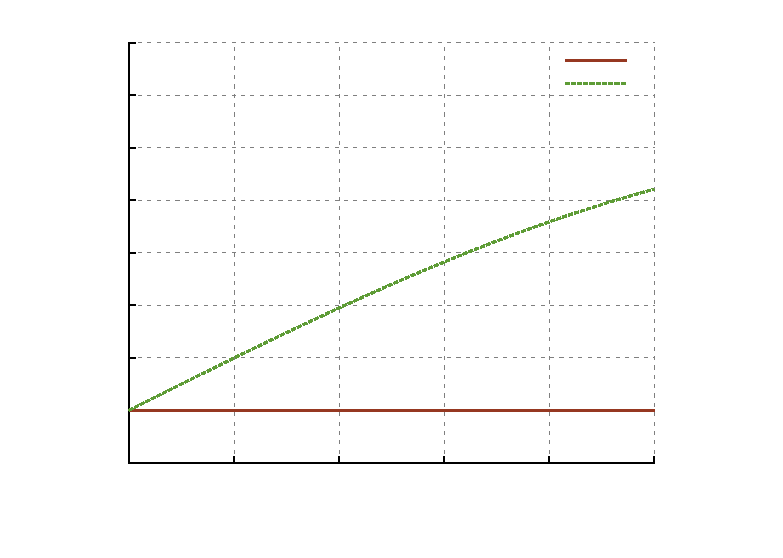
\includegraphics{sin}}%
    \gplfronttext
  \end{picture}%
\endgroup
}
	\caption{Solution over time}
	\label{fig:sin}
\end{figure}

Lorem ipsum dolor sit amet, consetetur sadipscing elitr, sed diam nonumy eirmod tempor invidunt ut labore et dolore magna aliquyam erat, sed diam voluptua. At vero eos et accusam et justo duo dolores et ea rebum. Stet clita kasd gubergren, no sea takimata sanctus est Lorem ipsum dolor sit amet. Lorem ipsum dolor sit amet, consetetur sadipscing elitr, sed diam nonumy eirmod tempor invidunt ut labore et dolore magna aliquyam erat, sed diam voluptua. At vero eos et accusam et justo duo dolores et ea rebum. Stet clita kasd gubergren, no sea takimata sanctus est Lorem ipsum dolor sit amet. see \Fref{tab:broyNewto}

\begin{table}[!htb]
	\caption{Behavior of the quasi Newton method... }
	\begin{center}
		\begin{tabular}{@{}n{2}{0} n{1}{16} n{1}{16} n{1}{16}@{}}\toprule
			\multicolumn{1}{@{}H}{iteration}& \multicolumn{1}{H}{$\left\| F\left(\leftidx{^{m}}x \right) \right\|$}& \multicolumn{1}{H}{$\left\| \leftidx{^{m}} \Delta x  \right\|$} & \multicolumn{1}{H@{}}{$\leftidx{^{m}}e_{\mathrm{fixP}}$} \tabularnewline\midrule\addlinespace
			%   &                     &                    &                    \tabularnewline\midrule\addlinespace
			0  & 1.4142135623730951  & 1.4142135623730951 & 0.3034928278335036 \tabularnewline
			1  & 0.4259168303185923  & 0.3273340629945428 & 0.0238412351610392 \tabularnewline
			2  & 0.0337150010756715  & 0.0240106701324139 & 0.0001694349713746 \tabularnewline
			3  & 0.0002396172338851  & 0.0001694429402329 & 0.0000000079688583 \tabularnewline
			4  & 0.0000000112696676  & 0.0000000079688584 & 0.0000000000000002 \tabularnewline\addlinespace\bottomrule
		\end{tabular}
	\end{center}
	\label{tab:broyNewton}
\end{table}

